\documentclass[10pt, a4paper, english]{article}\usepackage[]{graphicx}\usepackage[dvipsnames]{xcolor}
% maxwidth is the original width if it is less than linewidth
% otherwise use linewidth (to make sure the graphics do not exceed the margin)
\makeatletter
\def\maxwidth{ %
  \ifdim\Gin@nat@width>\linewidth
    \linewidth
  \else
    \Gin@nat@width
  \fi
}
\makeatother

\definecolor{fgcolor}{rgb}{0.345, 0.345, 0.345}
\newcommand{\hlnum}[1]{\textcolor[rgb]{0.686,0.059,0.569}{#1}}%
\newcommand{\hlstr}[1]{\textcolor[rgb]{0.192,0.494,0.8}{#1}}%
\newcommand{\hlcom}[1]{\textcolor[rgb]{0.678,0.584,0.686}{\textit{#1}}}%
\newcommand{\hlopt}[1]{\textcolor[rgb]{0,0,0}{#1}}%
\newcommand{\hlstd}[1]{\textcolor[rgb]{0.345,0.345,0.345}{#1}}%
\newcommand{\hlkwa}[1]{\textcolor[rgb]{0.161,0.373,0.58}{\textbf{#1}}}%
\newcommand{\hlkwb}[1]{\textcolor[rgb]{0.69,0.353,0.396}{#1}}%
\newcommand{\hlkwc}[1]{\textcolor[rgb]{0.333,0.667,0.333}{#1}}%
\newcommand{\hlkwd}[1]{\textcolor[rgb]{0.737,0.353,0.396}{\textbf{#1}}}%
\let\hlipl\hlkwb

\usepackage{framed}
\makeatletter
\newenvironment{kframe}{%
 \def\at@end@of@kframe{}%
 \ifinner\ifhmode%
  \def\at@end@of@kframe{\end{minipage}}%
  \begin{minipage}{\columnwidth}%
 \fi\fi%
 \def\FrameCommand##1{\hskip\@totalleftmargin \hskip-\fboxsep
 \colorbox{shadecolor}{##1}\hskip-\fboxsep
     % There is no \\@totalrightmargin, so:
     \hskip-\linewidth \hskip-\@totalleftmargin \hskip\columnwidth}%
 \MakeFramed {\advance\hsize-\width
   \@totalleftmargin\z@ \linewidth\hsize
   \@setminipage}}%
 {\par\unskip\endMakeFramed%
 \at@end@of@kframe}
\makeatother

\definecolor{shadecolor}{rgb}{.97, .97, .97}
\definecolor{messagecolor}{rgb}{0, 0, 0}
\definecolor{warningcolor}{rgb}{1, 0, 1}
\definecolor{errorcolor}{rgb}{1, 0, 0}
\newenvironment{knitrout}{}{} % an empty environment to be redefined in TeX

\usepackage{alltt}
%typesetting
\usepackage[margin = 1in]{geometry} % margins
\usepackage[T1]{fontenc} % font encoding
\usepackage{babel} %enables typesetting for multiple languages
\usepackage{parskip} %new lines
\usepackage{graphicx} 
\usepackage{float}
\floatplacement{figure}{H} %when printing tables, include  table.position="H"
\usepackage{bm}
\usepackage{amsmath}

\usepackage[dvipsnames]{xcolor} % more colors

\usepackage[colorlinks]{hyperref}


 %clickable table of contents from hyperref
\hypersetup{
    colorlinks,
    citecolor=black,
    filecolor=black,
    linkcolor=black,
    urlcolor=black
}

\usepackage[colorinlistoftodos]{todonotes}

\title{Machine Learning 2ST129 26605 HT2023
 Assignment 5}
\author{Anonymous Student}
\date{\today}
\IfFileExists{upquote.sty}{\usepackage{upquote}}{}
\begin{document}
\maketitle
\newpage
\tableofcontents
\newpage

\section*{General Information}
\begin{itemize}
\item Time used for reading: 2 hours
\item Time used for basic assignment 15 hours:
\item Time used for extra assignment 6 hours: 
\item Good with lab: Its good that you had the implement the steps one at a time, which helps with learning how the models works.
\item Things improve with lab: Since there is a newer version of Deep Learning with R, it would be nice if there were reading instructions for that version as well. 
\end{itemize}
\newpage




\begin{knitrout}
\definecolor{shadecolor}{rgb}{0.969, 0.969, 0.969}\color{fgcolor}\begin{kframe}
\begin{alltt}
\hlcom{#Libraries}
 \hlkwd{library}\hlstd{(tidyverse)}
 \hlkwd{library}\hlstd{(xtable)}
 \hlkwd{library}\hlstd{(tensorflow)}
 \hlkwd{library}\hlstd{(keras)}
 \hlkwd{library}\hlstd{(uuml)}
\end{alltt}
\end{kframe}
\end{knitrout}
\section{Task 1}
\subsection{1.1}
First we start computing the query, key and value matrices for one attention head by implementing it in a function \texttt{qkv()}

\begin{knitrout}
\definecolor{shadecolor}{rgb}{0.969, 0.969, 0.969}\color{fgcolor}\begin{kframe}
\begin{alltt}
\hlkwd{data}\hlstd{(}\hlstr{"transformer_example"}\hlstd{)}
 \hlstd{qkv} \hlkwb{<-} \hlkwa{function}\hlstd{(}\hlkwc{X}\hlstd{,} \hlkwc{Wq}\hlstd{,} \hlkwc{Wk}\hlstd{,} \hlkwc{Wv}\hlstd{)\{}
   \hlstd{Q}\hlkwb{<-} \hlstd{X} \hlopt \hlstd{Wq}
   \hlstd{K} \hlkwb{<-} \hlstd{X} \hlopt \hlstd{Wk}
   \hlstd{V} \hlkwb{<-} \hlstd{X} \hlopt \hlstd{Wv}
   \hlkwd{return}\hlstd{(}\hlkwd{list}\hlstd{(}\hlkwc{Q}\hlstd{=Q,} \hlkwc{K}\hlstd{=K,} \hlkwc{V}\hlstd{=V))}
 \hlstd{\}}


\hlstd{Wq} \hlkwb{<-} \hlstd{transformer_example}\hlopt{$}\hlstd{Wq[,,} \hlnum{1}\hlstd{]}
 \hlstd{Wk} \hlkwb{<-} \hlstd{transformer_example}\hlopt{$}\hlstd{Wk[,,} \hlnum{1}\hlstd{]}
 \hlstd{Wv} \hlkwb{<-} \hlstd{transformer_example}\hlopt{$}\hlstd{Wv[,,} \hlnum{1}\hlstd{]}
\hlstd{X} \hlkwb{<-} \hlstd{transformer_example}\hlopt{$}\hlstd{embeddings[}\hlnum{1}\hlopt{:} \hlnum{3}\hlstd{,]}

\hlstd{res} \hlkwb{<-} \hlkwd{qkv}\hlstd{(X, Wq, Wk, Wv)}
\end{alltt}
\end{kframe}
\end{knitrout}

  % We can now refer to it as Figure \ref{fig:my_plot}

\subsection{1.2}
Now, based on the query, key and value,  we want to compute the attention of that given attention head for the three chosen tokens. This procedures involes multiple steps. 

\begin{knitrout}
\definecolor{shadecolor}{rgb}{0.969, 0.969, 0.969}\color{fgcolor}\begin{kframe}
\begin{alltt}
\hlstd{softmax} \hlkwb{<-} \hlkwa{function}\hlstd{(}\hlkwc{X}\hlstd{)\{}
  \hlstd{value} \hlkwb{<-} \hlkwd{exp}\hlstd{(X)} \hlopt{/} \hlkwd{rowSums}\hlstd{(}\hlkwd{exp}\hlstd{(X))}
  \hlkwd{return}\hlstd{(value)}
  \hlstd{\}}
\hlstd{attention} \hlkwb{<-} \hlkwa{function}\hlstd{(}\hlkwc{Q}\hlstd{,} \hlkwc{K}\hlstd{,} \hlkwc{V}\hlstd{) \{}
  \hlstd{key_dim} \hlkwb{<-} \hlkwd{ncol}\hlstd{(K)}
  \hlstd{score_ratio} \hlkwb{<-} \hlstd{(Q}\hlopt \hlkwd{t}\hlstd{(K))} \hlopt{/} \hlkwd{sqrt}\hlstd{(key_dim)}

  \hlstd{attention} \hlkwb{<-} \hlkwd{softmax}\hlstd{(score_ratio)}


  \hlstd{Z} \hlkwb{<-} \hlstd{attention} \hlopt \hlstd{V}

  \hlstd{results} \hlkwb{<-} \hlkwd{list}\hlstd{(}\hlkwc{Z} \hlstd{= Z,} \hlkwc{attention} \hlstd{= attention)}
  \hlkwd{return}\hlstd{(results)}
\hlstd{\}}

\hlkwd{attention}\hlstd{(res}\hlopt{$}\hlstd{Q, res}\hlopt{$}\hlstd{K, res}\hlopt{$}\hlstd{V)}
\end{alltt}
\begin{verbatim}
$Z
              [,1]          [,2]         [,3]
the    0.012395453 -0.0212420459  0.009404870
quick -0.003759269 -0.0008360029 -0.005108890
brown  0.002412222 -0.0088974612  0.001147999

$attention
            the     quick     brown
the   0.3601932 0.3080896 0.3317172
quick 0.3088780 0.3582373 0.3328847
brown 0.3300375 0.3360583 0.3339042
\end{verbatim}
\end{kframe}
\end{knitrout}

\subsection{1.3}
The resulting vector is one we can send along to the feed-forward neural network.
The second row of the attention matrix, are the 
 attention scores assigned to the second token, or quick in this case, with respect to   
 with respect to all other tokens, including itself. For example, in the second row, the second element is the highest, which is the attention score of quick attending to itself. 

\subsection{1.4}
Now we will implement a multi-head attention layer.

\begin{knitrout}
\definecolor{shadecolor}{rgb}{0.969, 0.969, 0.969}\color{fgcolor}\begin{kframe}
\begin{alltt}
\hlstd{compute_attention} \hlkwb{<-} \hlkwa{function}\hlstd{(}\hlkwc{X}\hlstd{,} \hlkwc{Wq}\hlstd{,} \hlkwc{Wk}\hlstd{,} \hlkwc{Wv}\hlstd{)\{}
  \hlstd{qkv_res} \hlkwb{<-} \hlkwd{qkv}\hlstd{(X, Wq, Wk, Wv)}
  \hlstd{attention} \hlkwb{<-} \hlkwd{attention}\hlstd{(qkv_res}\hlopt{$}\hlstd{Q, qkv_res}\hlopt{$}\hlstd{K, qkv_res}\hlopt{$}\hlstd{V)}
  \hlkwd{return}\hlstd{(attention)}
\hlstd{\}}

\hlstd{multi_head_self_attention} \hlkwb{<-} \hlkwa{function}\hlstd{(}\hlkwc{X}\hlstd{,}\hlkwc{Q}\hlstd{,} \hlkwc{K} \hlstd{,} \hlkwc{V}\hlstd{,} \hlkwc{W0}\hlstd{)\{}
  \hlstd{n_weights} \hlkwb{<-} \hlkwd{dim}\hlstd{(K)[}\hlnum{3}\hlstd{]}
   \hlstd{attention_heads} \hlkwb{<-} \hlkwd{sapply}\hlstd{(}\hlnum{1}\hlopt{:}\hlstd{n_weights,} \hlkwc{FUN}\hlstd{=}\hlkwa{function}\hlstd{(}\hlkwc{i}\hlstd{)\{}
   \hlkwd{compute_attention}\hlstd{(X, Q[,,i], K[,,i], V[,,i])}
  \hlstd{\},} \hlkwc{simplify} \hlstd{=} \hlnum{FALSE}\hlstd{)}
  \hlstd{combined_matrix}\hlkwb{<-} \hlkwd{do.call}\hlstd{(cbind,} \hlkwd{lapply}\hlstd{(attention_heads,} \hlkwc{FUN} \hlstd{=} \hlkwa{function}\hlstd{(}\hlkwc{sub_list}\hlstd{)\{}
     \hlstd{sub_list}\hlopt{$}\hlstd{Z}
  \hlstd{\}))}
  \hlstd{results} \hlkwb{<-} \hlstd{combined_matrix} \hlopt \hlstd{W0}
  \hlkwd{return}\hlstd{(results)}
\hlstd{\}}
\end{alltt}
\end{kframe}
\end{knitrout}


\begin{knitrout}
\definecolor{shadecolor}{rgb}{0.969, 0.969, 0.969}\color{fgcolor}\begin{kframe}
\begin{alltt}
\hlcom{#on example data}
\hlkwd{multi_head_self_attention}\hlstd{(X,transformer_example}\hlopt{$}\hlstd{Wq, transformer_example}\hlopt{$}\hlstd{Wk,}
                                  \hlstd{transformer_example}\hlopt{$}\hlstd{Wv, transformer_example}\hlopt{$}\hlstd{W0)}
\end{alltt}
\begin{verbatim}
              [,1]          [,2]         [,3]
the   -0.014189613 -0.0040299008 -0.006756286
quick -0.009963516 -0.0010724342 -0.001996524
brown -0.006394562 -0.0006626115 -0.002219108
\end{verbatim}
\begin{alltt}
\hlcom{#On whole data}
\hlstd{X} \hlkwb{<-} \hlstd{transformer_example}\hlopt{$}\hlstd{embeddings}
\hlkwd{multi_head_self_attention}\hlstd{(X,transformer_example}\hlopt{$}\hlstd{Wq, transformer_example}\hlopt{$}\hlstd{Wk,}
                                  \hlstd{transformer_example}\hlopt{$}\hlstd{Wv, transformer_example}\hlopt{$}\hlstd{W0)}
\end{alltt}
\begin{verbatim}
             [,1]        [,2]       [,3]
the   -0.02705494 0.005860020 0.01218247
quick -0.02413116 0.008522431 0.02030744
brown -0.02158066 0.009040085 0.02021518
fox   -0.02744489 0.004881125 0.01531574
jumps -0.02348063 0.008342224 0.01498752
over  -0.02592150 0.006371230 0.01826652
the   -0.02705494 0.005860020 0.01218247
lazy  -0.02755128 0.006333208 0.02246126
dog   -0.02986621 0.005885128 0.01774406
\end{verbatim}
\end{kframe}
\end{knitrout}
\section{Task 2}
 
\subsection{Task 2.1}
 Now we are going to implement a one-layer recurrent neural network based on the rnn\_example data. First we implement a RNN linear unit. 
 
 
 
\begin{knitrout}
\definecolor{shadecolor}{rgb}{0.969, 0.969, 0.969}\color{fgcolor}\begin{kframe}
\begin{alltt}
\hlstd{X} \hlkwb{<-} \hlstd{rnn_example}\hlopt{$}\hlstd{embeddings[}\hlnum{1}\hlstd{,,} \hlkwc{drop}\hlstd{=}\hlnum{FALSE}\hlstd{]}
\hlstd{X}
\end{alltt}
\begin{verbatim}
        [,1]    [,2]     [,3]       [,4]       [,5]
the 1.819735 1.37044 1.196318 -0.4068792 -0.6109788
\end{verbatim}
\begin{alltt}
\hlstd{hidden_dim} \hlkwb{<-} \hlnum{4}

\hlstd{h_t_minus_one} \hlkwb{<-} \hlkwd{matrix}\hlstd{(}\hlnum{0}\hlstd{,} \hlkwc{nrow} \hlstd{= hidden_dim,} \hlkwc{ncol} \hlstd{=} \hlnum{1}\hlstd{)}

\hlstd{rnn_unit} \hlkwb{<-} \hlkwa{function}\hlstd{(}\hlkwc{W}\hlstd{,}\hlkwc{U}\hlstd{,}\hlkwc{b}\hlstd{,} \hlkwc{h_t_minus_one}\hlstd{,} \hlkwc{x_t}\hlstd{)\{}
  \hlstd{at} \hlkwb{<-} \hlstd{b} \hlopt{+} \hlstd{W} \hlopt \hlstd{h_t_minus_one} \hlopt{+} \hlstd{U} \hlopt \hlkwd{t}\hlstd{(x_t)}

  \hlkwd{return}\hlstd{(at)}
\hlstd{\}}

\hlstd{a_t} \hlkwb{<-} \hlkwd{rnn_unit}\hlstd{(h_t_minus_one,} \hlkwc{x_t}\hlstd{=X,} \hlkwc{W} \hlstd{= rnn_example}\hlopt{$}\hlstd{W,} \hlkwc{U} \hlstd{= rnn_example}\hlopt{$}\hlstd{U,} \hlkwc{b} \hlstd{= rnn_example}\hlopt{$}\hlstd{b)}
\hlstd{a_t}
\end{alltt}
\begin{verbatim}
            the
[1,]  0.5819145
[2,] -2.2686535
[3,] -0.6410312
[4,]  1.4891931
\end{verbatim}
\end{kframe}
\end{knitrout}

\subsection{2.2}
Now we implement the \texttt{tanh()} activation function $$\frac{e^x-e^{-x}}{e^x+e^{-x}}$$
\begin{knitrout}
\definecolor{shadecolor}{rgb}{0.969, 0.969, 0.969}\color{fgcolor}\begin{kframe}
\begin{alltt}
\hlstd{activation} \hlkwb{<-} \hlkwa{function}\hlstd{(}\hlkwc{x}\hlstd{)\{}
  \hlkwd{return}\hlstd{((}\hlkwd{exp}\hlstd{(x)} \hlopt{-} \hlkwd{exp}\hlstd{(}\hlopt{-}\hlstd{x))} \hlopt{/} \hlstd{(}\hlkwd{exp}\hlstd{(x)} \hlopt{+} \hlkwd{exp}\hlstd{(}\hlopt{-}\hlstd{x)))}
\hlstd{\}}

\hlstd{h_t} \hlkwb{<-} \hlkwd{activation}\hlstd{(a_t)}

\hlstd{h_t}
\end{alltt}
\begin{verbatim}
            the
[1,]  0.5240555
[2,] -0.9788223
[3,] -0.5656013
[4,]  0.9031762
\end{verbatim}
\end{kframe}
\end{knitrout}


\subsection{2.3}
Now to implement the output function and the softmax function.

\begin{knitrout}
\definecolor{shadecolor}{rgb}{0.969, 0.969, 0.969}\color{fgcolor}\begin{kframe}
\begin{alltt}
\hlstd{output_rnn}\hlkwb{<-} \hlkwa{function}\hlstd{(}\hlkwc{h_t}\hlstd{,} \hlkwc{V}\hlstd{,} \hlkwc{c}\hlstd{)\{}
  \hlkwd{return}\hlstd{(c} \hlopt{+} \hlstd{V} \hlopt \hlstd{h_t)}
\hlstd{\}}
\hlstd{softmax} \hlkwb{<-} \hlkwa{function}\hlstd{(}\hlkwc{o}\hlstd{)\{}
  \hlkwd{return}\hlstd{(}\hlkwd{exp}\hlstd{(o)} \hlopt{/} \hlkwd{sum}\hlstd{(}\hlkwd{exp}\hlstd{(o)))}
\hlstd{\}}


\hlkwd{softmax}\hlstd{(}\hlkwd{output_rnn}\hlstd{(h_t, rnn_example}\hlopt{$}\hlstd{V, rnn_example}\hlopt{$}\hlstd{c) )}
\end{alltt}
\begin{verbatim}
           the
[1,] 0.3063613
[2,] 0.2930885
[3,] 0.4005502
\end{verbatim}
\end{kframe}
\end{knitrout}

\subsection{2.4}

Now we implement the full recurrent layer. 
\begin{knitrout}
\definecolor{shadecolor}{rgb}{0.969, 0.969, 0.969}\color{fgcolor}\begin{kframe}
\begin{alltt}
\hlcom{#' combines all the previous functions in one function}
\hlstd{rnn_combined} \hlkwb{<-} \hlkwa{function}\hlstd{(}\hlkwc{X}\hlstd{,} \hlkwc{W}\hlstd{,} \hlkwc{V}\hlstd{,} \hlkwc{U}\hlstd{,} \hlkwc{b}\hlstd{,} \hlkwc{c}\hlstd{,} \hlkwc{hidden_dim} \hlstd{=} \hlnum{4}\hlstd{,} \hlkwc{h_t_minus_one}\hlstd{) \{}
  \hlstd{a_t} \hlkwb{<-} \hlkwd{rnn_unit}\hlstd{(}\hlkwc{h_t_minus_one} \hlstd{= h_t_minus_one,} \hlkwc{W} \hlstd{= W,} \hlkwc{U} \hlstd{= U,} \hlkwc{b} \hlstd{= b,} \hlkwc{x_t} \hlstd{= X)}
  \hlstd{ht} \hlkwb{<-} \hlkwd{activation}\hlstd{(a_t)}
  \hlstd{o} \hlkwb{<-} \hlkwd{output_rnn}\hlstd{(ht, V, c)}

  \hlstd{y_hat} \hlkwb{<-} \hlkwd{softmax}\hlstd{(o)}
  \hlkwd{return}\hlstd{(}\hlkwd{list}\hlstd{(}\hlkwc{ht} \hlstd{= ht,} \hlkwc{y_hat} \hlstd{= y_hat))}
\hlstd{\}}


\hlcom{#Assuming the words are the rows of X}
\hlstd{rnn_layer} \hlkwb{<-} \hlkwa{function}\hlstd{(}\hlkwc{X}\hlstd{,} \hlkwc{W}\hlstd{,} \hlkwc{V}\hlstd{,} \hlkwc{U}\hlstd{,} \hlkwc{b}\hlstd{,} \hlkwc{c}\hlstd{,} \hlkwc{hidden_dim} \hlstd{=} \hlnum{4}\hlstd{)\{}
  \hlstd{n_rows} \hlkwb{<-} \hlkwd{nrow}\hlstd{(X)}
  \hlstd{h_t_minus_one} \hlkwb{<-} \hlkwd{matrix}\hlstd{(}\hlnum{0}\hlstd{,} \hlkwc{nrow} \hlstd{= hidden_dim,} \hlkwc{ncol} \hlstd{=} \hlnum{1}\hlstd{)}
  \hlstd{h_t} \hlkwb{<-} \hlkwd{matrix}\hlstd{(}\hlnum{NA}\hlstd{,} \hlkwc{ncol}\hlstd{=hidden_dim,} \hlkwc{nrow}\hlstd{=n_rows)}
  \hlstd{y_hat} \hlkwb{<-} \hlkwd{matrix}\hlstd{(}\hlnum{NA}\hlstd{,} \hlkwc{ncol}\hlstd{=}\hlkwd{nrow}\hlstd{(V),} \hlkwc{nrow}\hlstd{=n_rows)}
  \hlkwa{for}\hlstd{(i} \hlkwa{in} \hlnum{1}\hlopt{:}\hlstd{n_rows)\{}
    \hlstd{X_subset} \hlkwb{<-} \hlstd{X[i,,} \hlkwc{drop}\hlstd{=}\hlnum{FALSE}\hlstd{]}
    \hlstd{iter_res} \hlkwb{<-} \hlkwd{rnn_combined}\hlstd{(X_subset, W, V, U, b, c, hidden_dim, h_t_minus_one)}
    \hlstd{h_t_minus_one} \hlkwb{<-} \hlstd{h_t[i,]} \hlkwb{<-} \hlstd{iter_res}\hlopt{$}\hlstd{ht}
    \hlstd{y_hat[i,]} \hlkwb{<-} \hlstd{iter_res}\hlopt{$}\hlstd{y_hat}
  \hlstd{\}}
  \hlkwd{rownames}\hlstd{(h_t)} \hlkwb{<-} \hlkwd{rownames}\hlstd{(y_hat)} \hlkwb{<-} \hlkwd{rownames}\hlstd{(X)}
  \hlstd{list} \hlkwb{<-} \hlkwd{list}\hlstd{(}\hlkwc{ht}\hlstd{=h_t,} \hlkwc{y_hat} \hlstd{= y_hat)}
  \hlkwd{return}\hlstd{(list)}
\hlstd{\}}

\hlcom{#checking that it works for both cases}

\hlkwd{rnn_layer}\hlstd{(X,} \hlkwc{W} \hlstd{= rnn_example}\hlopt{$}\hlstd{W,} \hlkwc{V} \hlstd{= rnn_example}\hlopt{$}\hlstd{V,}
          \hlkwc{U} \hlstd{= rnn_example}\hlopt{$}\hlstd{U, rnn_example}\hlopt{$}\hlstd{b,}\hlkwc{c}\hlstd{=  rnn_example}\hlopt{$}\hlstd{c)}
\end{alltt}
\begin{verbatim}
$ht
         [,1]       [,2]       [,3]      [,4]
the 0.5240555 -0.9788223 -0.5656013 0.9031762

$y_hat
         [,1]      [,2]      [,3]
the 0.3063613 0.2930885 0.4005502
\end{verbatim}
\begin{alltt}
\hlstd{X_new} \hlkwb{<-} \hlstd{rnn_example}\hlopt{$}\hlstd{embeddings[}\hlnum{1}\hlopt{:} \hlnum{3}\hlstd{,,} \hlkwc{drop}\hlstd{=}\hlnum{FALSE}\hlstd{]}

\hlkwd{rnn_layer}\hlstd{(X_new,} \hlkwc{W} \hlstd{= rnn_example}\hlopt{$}\hlstd{W,} \hlkwc{V} \hlstd{= rnn_example}\hlopt{$}\hlstd{V,}
          \hlkwc{U} \hlstd{= rnn_example}\hlopt{$}\hlstd{U, rnn_example}\hlopt{$}\hlstd{b,}\hlkwc{c}\hlstd{=  rnn_example}\hlopt{$}\hlstd{c)}
\end{alltt}
\begin{verbatim}
$ht
             [,1]        [,2]       [,3]       [,4]
the    0.52405551 -0.97882227 -0.5656013  0.9031762
quick -0.05951368  0.03988226  0.8241800 -0.6562744
brown -0.08984008  0.92822217 -0.1563247 -0.6657626

$y_hat
           [,1]      [,2]      [,3]
the   0.3063613 0.2930885 0.4005502
quick 0.2838013 0.3490452 0.3671536
brown 0.2878002 0.3666877 0.3455121
\end{verbatim}
\end{kframe}
\end{knitrout}

\subsection{2.5}
Now we apply the function on the whole data and get the value of the hidden state for the token dog. 

\begin{knitrout}
\definecolor{shadecolor}{rgb}{0.969, 0.969, 0.969}\color{fgcolor}\begin{kframe}
\begin{alltt}
\hlstd{results} \hlkwb{<-} \hlkwd{rnn_layer}\hlstd{(}\hlkwc{X}\hlstd{= rnn_example}\hlopt{$}\hlstd{embeddings,} \hlkwc{W} \hlstd{= rnn_example}\hlopt{$}\hlstd{W,} \hlkwc{V} \hlstd{= rnn_example}\hlopt{$}\hlstd{V,}
          \hlkwc{U} \hlstd{= rnn_example}\hlopt{$}\hlstd{U, rnn_example}\hlopt{$}\hlstd{b,}\hlkwc{c}\hlstd{=  rnn_example}\hlopt{$}\hlstd{c)}

\hlstd{results}
\end{alltt}
\begin{verbatim}
$ht
             [,1]        [,2]       [,3]        [,4]
the    0.52405551 -0.97882227 -0.5656013  0.90317617
quick -0.05951368  0.03988226  0.8241800 -0.65627443
brown -0.08984008  0.92822217 -0.1563247 -0.66576260
fox   -0.43750124 -0.38442420  0.6070560  0.64156809
jumps  0.54934775 -0.24515537 -0.8748765  0.76466178
over  -0.62799359  0.82990292  0.6111049 -0.07918235
the    0.60957979 -0.97665249 -0.5596029  0.92482999
lazy  -0.92042949  0.90472482  0.9904783  0.03534373
dog   -0.29284645  0.18138447 -0.2190118  0.25923968

$y_hat
           [,1]      [,2]      [,3]
the   0.3063613 0.2930885 0.4005502
quick 0.2838013 0.3490452 0.3671536
brown 0.2878002 0.3666877 0.3455121
fox   0.2968252 0.3386681 0.3645066
jumps 0.3098598 0.3095035 0.3806367
over  0.2896910 0.3795378 0.3307712
the   0.3075896 0.2913470 0.4010634
lazy  0.2880155 0.3908604 0.3211241
dog   0.2956745 0.3461530 0.3581725
\end{verbatim}
\begin{alltt}
\hlstd{results}\hlopt{$}\hlstd{ht[}\hlstr{"dog"}\hlstd{, ,} \hlkwc{drop} \hlstd{=} \hlnum{FALSE}\hlstd{]}
\end{alltt}
\begin{verbatim}
          [,1]      [,2]       [,3]      [,4]
dog -0.2928465 0.1813845 -0.2190118 0.2592397
\end{verbatim}
\end{kframe}
\end{knitrout}


\section{Task 3}
\subsection{3.1}
First we load the data.
\begin{knitrout}
\definecolor{shadecolor}{rgb}{0.969, 0.969, 0.969}\color{fgcolor}\begin{kframe}
\begin{alltt}
\hlstd{imdb} \hlkwb{<-} \hlkwd{dataset_imdb}\hlstd{(}\hlkwc{num_words} \hlstd{=} \hlnum{10000}\hlstd{)} \hlcom{# we consider 10000 words as featers}
\hlstd{maxlen} \hlkwb{<-} \hlnum{20} \hlcom{#cut off the text after 20 words}
\hlkwd{c}\hlstd{(}\hlkwd{c}\hlstd{(input_train, y_train),} \hlkwd{c}\hlstd{(input_test, y_test))} \hlopt \hlstd{imdb}
\hlstd{input_train} \hlkwb{<-} \hlkwd{pad_sequences}\hlstd{(input_train,} \hlkwc{maxlen} \hlstd{= maxlen)} \hlcom{#load data as list of integers}
\hlstd{input_test} \hlkwb{<-} \hlkwd{pad_sequences}\hlstd{(input_test,} \hlkwc{maxlen} \hlstd{= maxlen)} \hlcom{#turn the list of integers into a 2D integer tensor of shape}
\end{alltt}
\end{kframe}
\end{knitrout}

Now to create a neural network using the following: 
\begin{itemize}
\item Emedding layer with 16 dimension
\item Hidden layer with 32 hidden stats
\item Validation split of 20 percent
\item batch size of 128
\item rmsprop and binary cross-entropy
\end{itemize}

\begin{knitrout}
\definecolor{shadecolor}{rgb}{0.969, 0.969, 0.969}\color{fgcolor}\begin{kframe}
\begin{alltt}
\hlstd{model} \hlkwb{<-} \hlkwd{keras_model_sequential}\hlstd{()} \hlopt
  \hlkwd{layer_embedding}\hlstd{(}\hlkwc{input_dim} \hlstd{=} \hlnum{10000}\hlstd{,} \hlkwc{output_dim} \hlstd{=} \hlnum{16}\hlstd{,}
                  \hlkwc{input_length} \hlstd{= maxlen)} \hlopt
  \hlkwd{layer_flatten}\hlstd{()} \hlopt
  \hlkwd{layer_dense}\hlstd{(}\hlkwc{units} \hlstd{=} \hlnum{32}\hlstd{,} \hlkwc{activation} \hlstd{=} \hlstr{"relu"}\hlstd{)} \hlopt
  \hlkwd{layer_dense}\hlstd{(}\hlkwc{units} \hlstd{=} \hlnum{1}\hlstd{,} \hlkwc{activation} \hlstd{=} \hlstr{"sigmoid"}\hlstd{)}

\hlkwd{summary}\hlstd{(model)}
\end{alltt}
\begin{verbatim}
Model: "sequential"
________________________________________________________________________________
 Layer (type)                       Output Shape                    Param #     
================================================================================
 embedding (Embedding)              (None, 20, 16)                  160000      
 flatten (Flatten)                  (None, 320)                     0           
 dense_1 (Dense)                    (None, 32)                      10272       
 dense (Dense)                      (None, 1)                       33          
================================================================================
Total params: 170305 (665.25 KB)
Trainable params: 170305 (665.25 KB)
Non-trainable params: 0 (0.00 Byte)
________________________________________________________________________________
\end{verbatim}
\end{kframe}
\end{knitrout}

\begin{knitrout}
\definecolor{shadecolor}{rgb}{0.969, 0.969, 0.969}\color{fgcolor}\begin{kframe}
\begin{alltt}
  \hlstd{model} \hlopt \hlkwd{compile}\hlstd{(}
  \hlkwc{optimizer} \hlstd{=} \hlstr{"rmsprop"}\hlstd{,}
  \hlkwc{loss} \hlstd{=} \hlstr{"binary_crossentropy"}\hlstd{,}
  \hlkwc{metrics} \hlstd{=} \hlkwd{c}\hlstd{(}\hlstr{"acc"}\hlstd{)}
\hlstd{)}



\hlstd{history} \hlkwb{<-} \hlstd{model} \hlopt \hlkwd{fit}\hlstd{(}
  \hlstd{input_train, y_train,}
  \hlkwc{epochs} \hlstd{=} \hlnum{10}\hlstd{,}
  \hlkwc{batch_size} \hlstd{=} \hlnum{128}\hlstd{,}
  \hlkwc{validation_split} \hlstd{=} \hlnum{0.2}
\hlstd{)}
\end{alltt}
\end{kframe}
\end{knitrout}


The result for the last epoch is:
\begin{knitrout}
\definecolor{shadecolor}{rgb}{0.969, 0.969, 0.969}\color{fgcolor}\begin{kframe}
\begin{alltt}
Epoch 10/10
157/157 [==============================] - 1s 3ms/step 
- loss: 0.0532 - acc: 0.9866 - val_loss: 0.9352 - val_acc: 0.7142
\end{alltt}
\end{kframe}
\end{knitrout}

\begin{knitrout}
\definecolor{shadecolor}{rgb}{0.969, 0.969, 0.969}\color{fgcolor}\begin{kframe}
\begin{alltt}
\hlstd{knitr}\hlopt{::}\hlkwd{include_graphics}\hlstd{(}\hlstr{"model1.png"}\hlstd{)}
\end{alltt}
\end{kframe}\begin{figure}
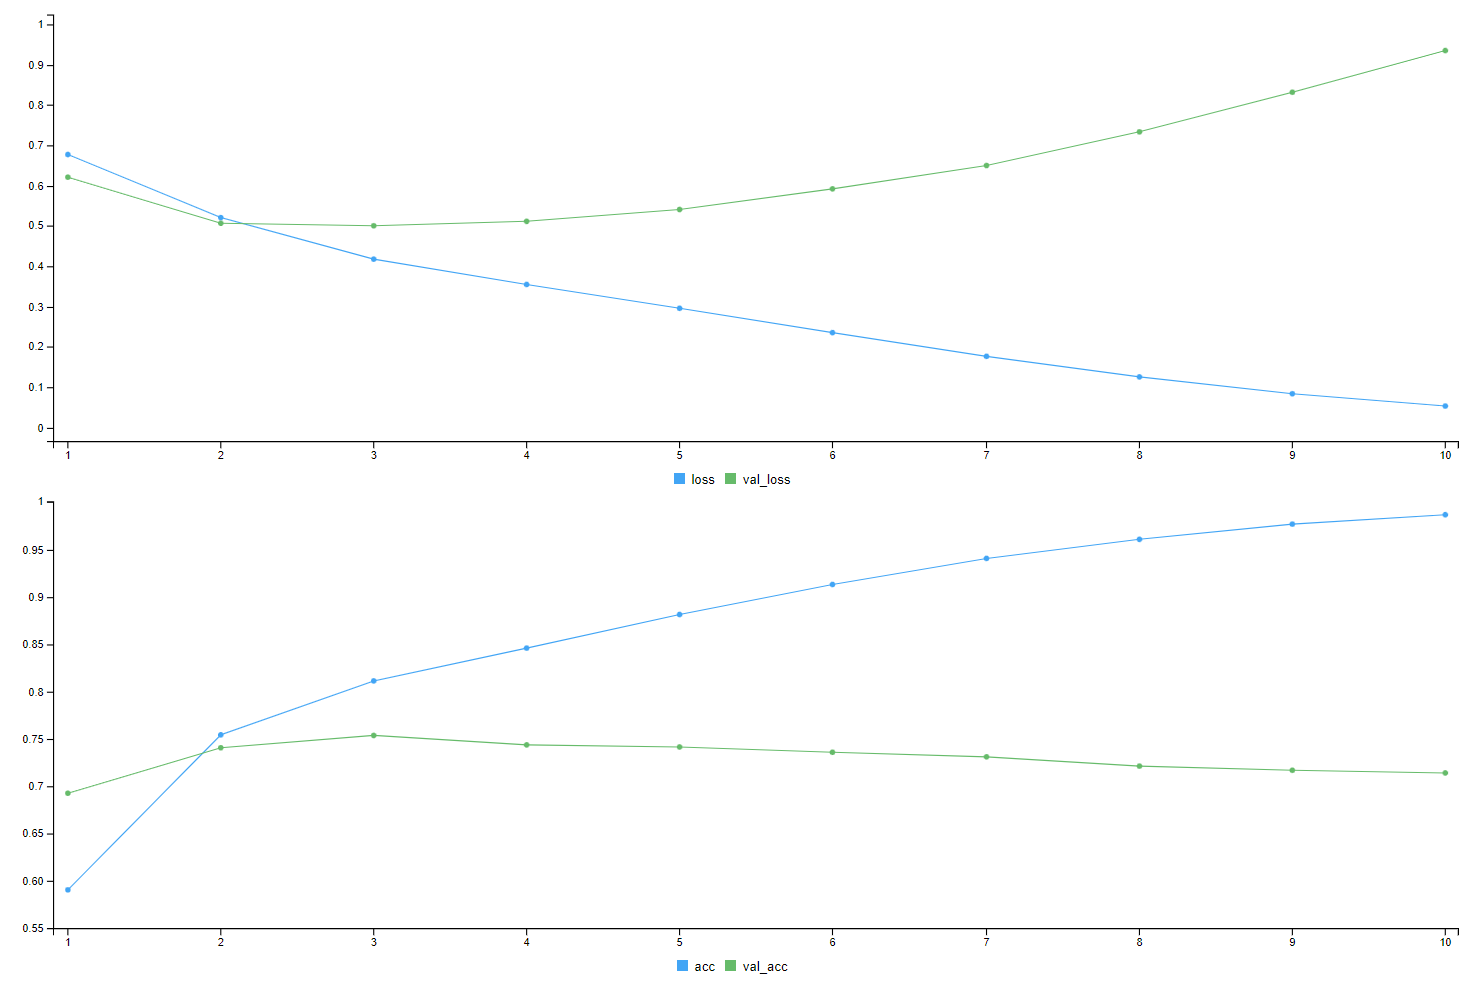
\includegraphics[width=\maxwidth]{model1} \caption[Results for the first model]{Results for the first model}\label{fig:unnamed-chunk-15}
\end{figure}

\end{knitrout}

As can be seen from the results, the validation accuracy for the last epoch is 0.7142.
\subsection{3.2}
The embedding layer uses two arguments, the number of possible tokens, which in this case equals to 10000 by the input\_dim,  and the dimension of the embedding as 16, as given by the output\_dim.
It can be seen as a dictionary such that it the indices for the integers are mapped to dense vectors. During its training process, it learns to associate each token or word with a specific vector. Then 
it works by using the input integers and searching for these integers in its internal dictionary and then return the corresponding vectors. 

\subsection{3.3}
Now to setup a simple RNN with 32 hidden units based on the same embedding layer. 

\begin{knitrout}
\definecolor{shadecolor}{rgb}{0.969, 0.969, 0.969}\color{fgcolor}\begin{kframe}
\begin{alltt}
\hlkwd{library}\hlstd{(keras)}

\hlstd{model2} \hlkwb{<-} \hlkwd{keras_model_sequential}\hlstd{()} \hlopt
  \hlkwd{layer_embedding}\hlstd{(}\hlkwc{input_dim} \hlstd{=} \hlnum{10000}\hlstd{,} \hlkwc{output_dim} \hlstd{=} \hlnum{16}\hlstd{,} \hlkwc{input_length} \hlstd{= maxlen)} \hlopt
  \hlkwd{layer_simple_rnn}\hlstd{(}\hlkwc{units} \hlstd{=} \hlnum{32}\hlstd{,} \hlkwc{activation} \hlstd{=} \hlstr{"tanh"}\hlstd{)} \hlopt  \hlcom{# RNN layer with 32 hidden units}
  \hlkwd{layer_dense}\hlstd{(}\hlkwc{units} \hlstd{=} \hlnum{1}\hlstd{,} \hlkwc{activation} \hlstd{=} \hlstr{"sigmoid"}\hlstd{)}

\hlkwd{summary}\hlstd{(model2)}
\end{alltt}
\begin{verbatim}
Model: "sequential_1"
________________________________________________________________________________
 Layer (type)                       Output Shape                    Param #     
================================================================================
 embedding_1 (Embedding)            (None, 20, 16)                  160000      
 simple_rnn (SimpleRNN)             (None, 32)                      1568        
 dense_2 (Dense)                    (None, 1)                       33          
================================================================================
Total params: 161601 (631.25 KB)
Trainable params: 161601 (631.25 KB)
Non-trainable params: 0 (0.00 Byte)
________________________________________________________________________________
\end{verbatim}
\end{kframe}
\end{knitrout}

\begin{knitrout}
\definecolor{shadecolor}{rgb}{0.969, 0.969, 0.969}\color{fgcolor}\begin{kframe}
\begin{alltt}
\hlstd{model2} \hlopt \hlkwd{compile}\hlstd{(}
  \hlkwc{optimizer} \hlstd{=} \hlstr{"rmsprop"}\hlstd{,}
  \hlkwc{loss} \hlstd{=} \hlstr{"binary_crossentropy"}\hlstd{,}
  \hlkwc{metrics} \hlstd{=} \hlkwd{c}\hlstd{(}\hlstr{"acc"}\hlstd{)}
\hlstd{)}

\hlstd{history2} \hlkwb{<-} \hlstd{model2} \hlopt \hlkwd{fit}\hlstd{(}
  \hlstd{input_train, y_train,}
  \hlkwc{epochs} \hlstd{=} \hlnum{10}\hlstd{,}
  \hlkwc{batch_size} \hlstd{=} \hlnum{128}\hlstd{,}
  \hlkwc{validation_split} \hlstd{=} \hlnum{0.2}
\hlstd{)}
\end{alltt}
\end{kframe}
\end{knitrout}

Now the results are:
\begin{knitrout}
\definecolor{shadecolor}{rgb}{0.969, 0.969, 0.969}\color{fgcolor}\begin{kframe}
\begin{alltt}
Epoch 10/10
157/157 [==============================] - 1s 5ms/step 
- loss: 0.0594 - acc: 0.9823 - val_loss: 1.0662 - val_acc: 0.6924
\end{alltt}
\end{kframe}
\end{knitrout}

\begin{knitrout}
\definecolor{shadecolor}{rgb}{0.969, 0.969, 0.969}\color{fgcolor}\begin{kframe}
\begin{alltt}
\hlstd{knitr}\hlopt{::}\hlkwd{include_graphics}\hlstd{(}\hlstr{"rnn_model.png"}\hlstd{)}
\end{alltt}
\end{kframe}\begin{figure}
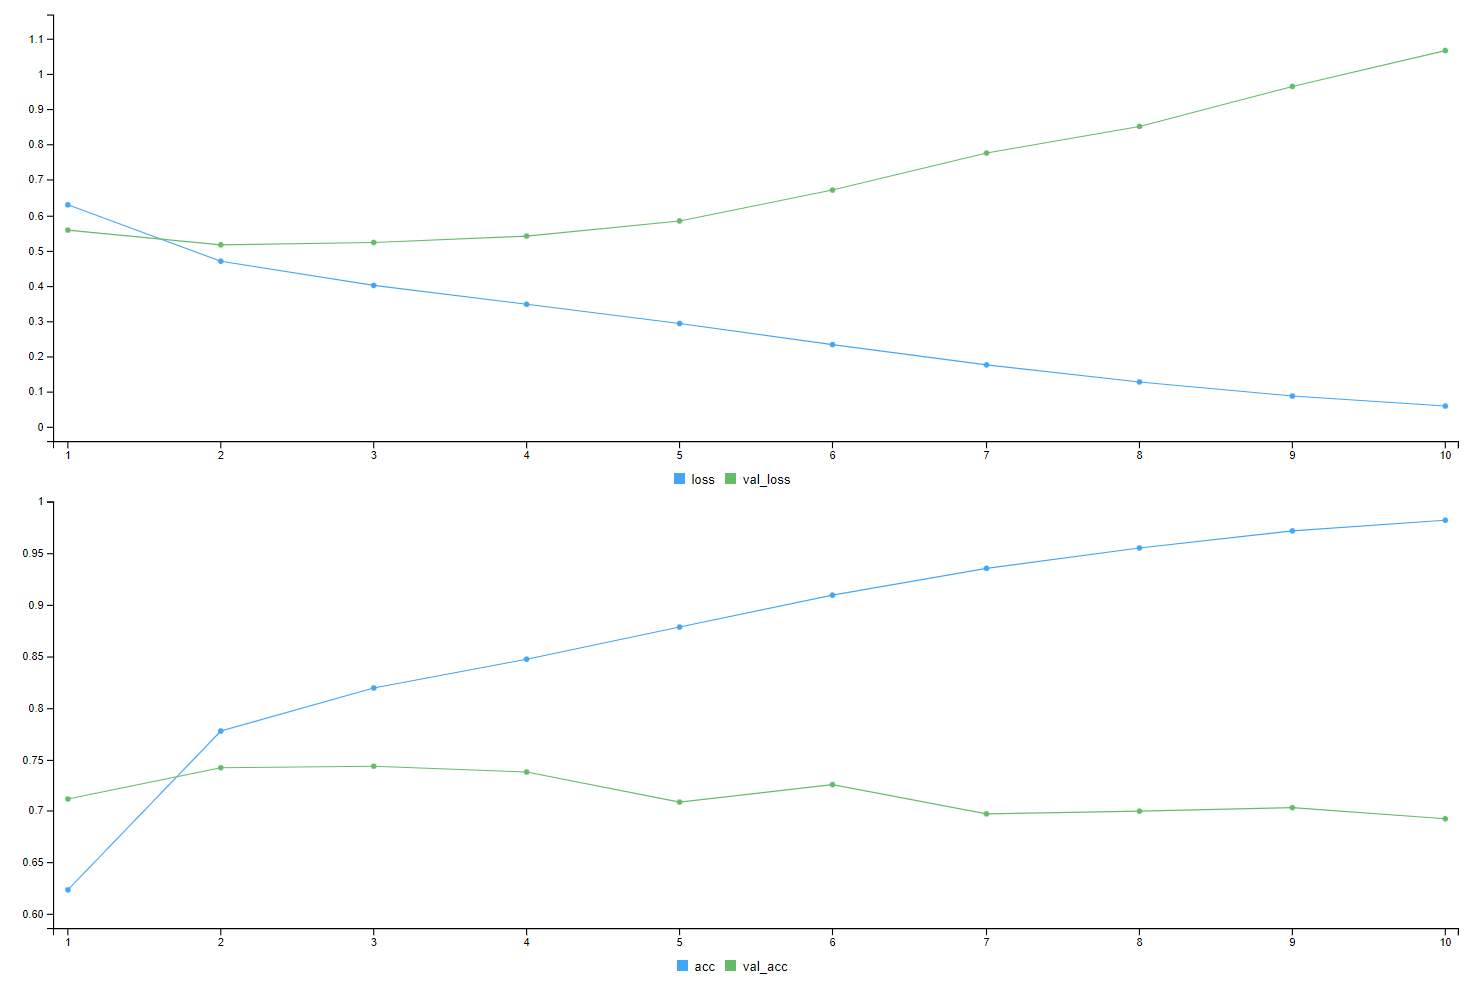
\includegraphics[width=\maxwidth]{rnn_model} \caption[Results for RNN model]{Results for RNN model}\label{fig:unnamed-chunk-19}
\end{figure}

\end{knitrout}
Now the validation accuracy is 0.6924. Hence this small rnn does not perform any better. Potentially it could be to the relatively small input length. 


\subsection{3.4}
The model implemented is best described by Fig. 10.5 in Goodfellow et al. The reason is that this model corresponds to a time/unfolded recurrent network with a single output at the end of the sequence, while also having recurrent connections among the hidden units. 
This is in contrast to the figure in 10.3 where the recurrent networks have recurrent connections among the hidden units, while producing an output at each time point \emph{t}. For example, in this model we have a dense layer with one unit, which means that the rnn gives a single output in the end. 

\subsection{3.5}
The matrix \textbf{U} in a RNN is a weight matrix representing the hidden connections from the input to the hidden state. The individual elements in the matrix, $U_{i_j}$ are the weights of the connection from a specific input feature $j$  to the \emph{i}:th hidden unit.   The matrix \textbf{W} is a weight matrix  for hidden-to-hidden connections. Here, each element $W_{i,j}$ represents the weight of the connection from the \emph{j}:th hidden unit at the previous time time periods to the \emph{i}:th hidden unit for the current time period. Hence \textbf{U} is related to the influence of the current input on the hidden state, whereas \textbf{W} is related to the influence of the previous hidden stat on the current hidden state. 


In the model above, these wight matrices are not directly viewable. However, they exist within the embedding layer. The total number of parameters in this case is the inut\_dim $\times$ output\_dim which equals to $10000 \times 16 = 160000$ for U. 

In the simple RNN layer \texttt{layer\_simple\_rnn()} we have $32 \times 32 + 16 \times 32 + 32 = 1568$ parameters, which contains both U and W.  


\subsection{3.6}
The parameters V represents hidden-to-output connections, or the connections from the recurrent layer to the dense layer, which computes the final output. The number of parameters here is dependent on the number of units ht the simple RNN layer as well as the number of units in the dense layer. Here we have that the number of parameters equals to $32 \times 1 + 1 = 33$where 32 is the number of units in the simple RNN layer and 1 is the number of units the the dense layer, as well as an additional 1 for the bias. 

\subsection{3.7}
New to implement a Long Short-Term Memory (LSTM) layer with 32 hidden units. 

\begin{knitrout}
\definecolor{shadecolor}{rgb}{0.969, 0.969, 0.969}\color{fgcolor}\begin{kframe}
\begin{alltt}
\hlstd{LSTM_model} \hlkwb{<-} \hlkwd{keras_model_sequential}\hlstd{()} \hlopt
  \hlkwd{layer_embedding}\hlstd{(}\hlkwc{input_dim} \hlstd{=} \hlnum{10000}\hlstd{,} \hlkwc{output_dim} \hlstd{=} \hlnum{16}\hlstd{)} \hlopt
  \hlkwd{layer_lstm}\hlstd{(}\hlkwc{units} \hlstd{=} \hlnum{32}\hlstd{)} \hlopt
  \hlkwd{layer_dense}\hlstd{(}\hlkwc{units} \hlstd{=} \hlnum{1}\hlstd{,} \hlkwc{activation} \hlstd{=} \hlstr{"sigmoid"}\hlstd{)}
\hlkwd{summary}\hlstd{(LSTM_model)}
\end{alltt}
\begin{verbatim}
Model: "sequential_2"
________________________________________________________________________________
 Layer (type)                       Output Shape                    Param #     
================================================================================
 embedding_2 (Embedding)            (None, None, 16)                160000      
 lstm (LSTM)                        (None, 32)                      6272        
 dense_3 (Dense)                    (None, 1)                       33          
================================================================================
Total params: 166305 (649.63 KB)
Trainable params: 166305 (649.63 KB)
Non-trainable params: 0 (0.00 Byte)
________________________________________________________________________________
\end{verbatim}
\end{kframe}
\end{knitrout}

\begin{knitrout}
\definecolor{shadecolor}{rgb}{0.969, 0.969, 0.969}\color{fgcolor}\begin{kframe}
\begin{alltt}
\hlstd{LSTM_model} \hlopt \hlkwd{compile}\hlstd{(}
  \hlkwc{optimizer} \hlstd{=} \hlstr{"rmsprop"}\hlstd{,}
  \hlkwc{loss} \hlstd{=} \hlstr{"binary_crossentropy"}\hlstd{,}
  \hlkwc{metrics} \hlstd{=} \hlkwd{c}\hlstd{(}\hlstr{"acc"}\hlstd{)}
\hlstd{)}
\hlstd{history_LSTM} \hlkwb{<-} \hlstd{LSTM_model} \hlopt \hlkwd{fit}\hlstd{(}
  \hlstd{input_train, y_train,}
  \hlkwc{epochs} \hlstd{=} \hlnum{10}\hlstd{,}
  \hlkwc{batch_size} \hlstd{=} \hlnum{128}\hlstd{,}
  \hlkwc{validation_split} \hlstd{=} \hlnum{0.2}
\hlstd{)}
\end{alltt}
\end{kframe}
\end{knitrout}


The results for the last epoch are:
\begin{knitrout}
\definecolor{shadecolor}{rgb}{0.969, 0.969, 0.969}\color{fgcolor}\begin{kframe}
\begin{alltt}
Epoch 10/10
157/157 [==============================] - 2s 12ms/step 
- loss: 0.2800 - acc: 0.8872 - val_loss: 0.5823 - val_acc: 0.7452
\end{alltt}
\end{kframe}
\end{knitrout}
The validation accuracy is 0.7452.
And the history of the results across all epochs:
\begin{knitrout}
\definecolor{shadecolor}{rgb}{0.969, 0.969, 0.969}\color{fgcolor}\begin{kframe}
\begin{alltt}
\hlstd{knitr}\hlopt{::}\hlkwd{include_graphics}\hlstd{(}\hlstr{"LSTM_model1.png"}\hlstd{)}
\end{alltt}
\end{kframe}\begin{figure}
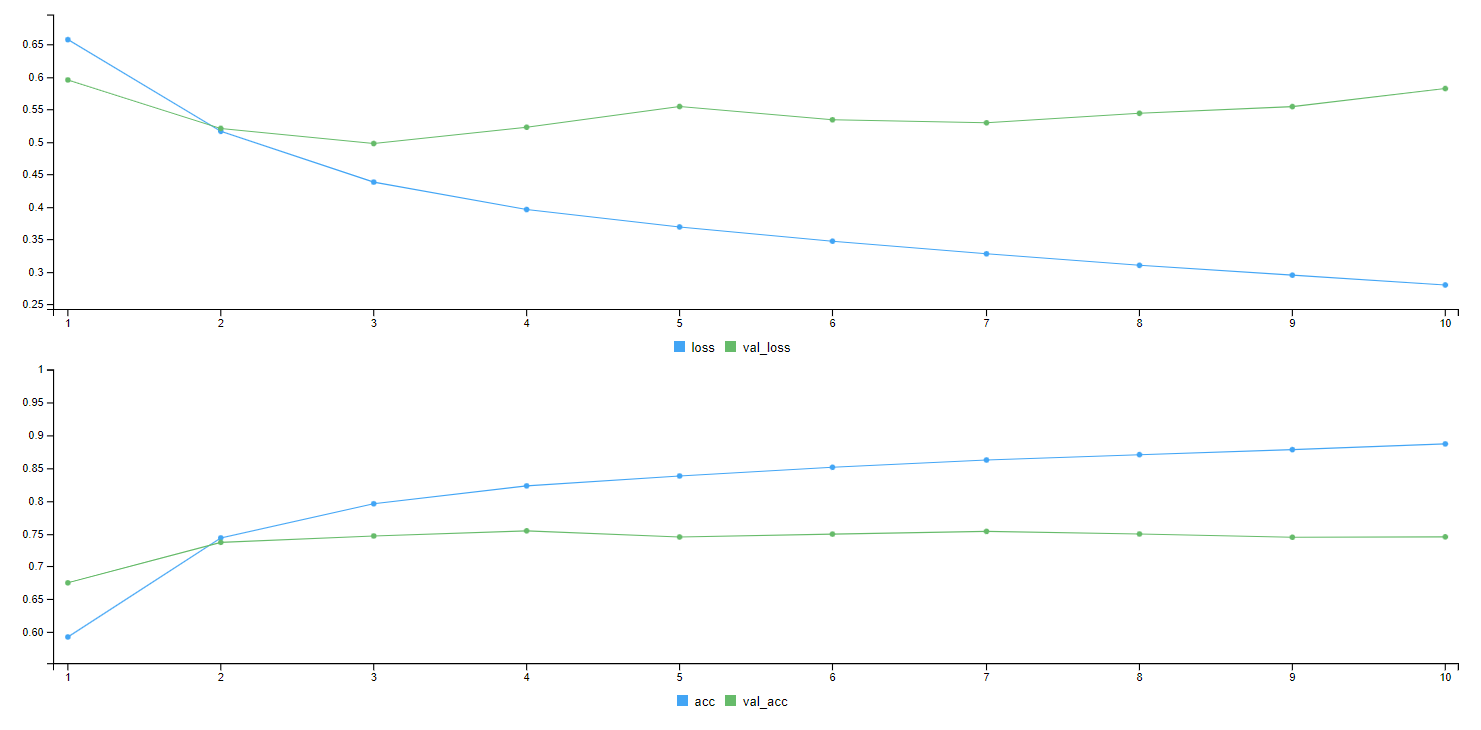
\includegraphics[width=\maxwidth]{LSTM_model1} \caption[Results for first LSTM model]{Results for first LSTM model}\label{fig:unnamed-chunk-23}
\end{figure}

\end{knitrout}

\section{3.8}
First we increase the number of words used to considers as features to 100 instead of 20. Then we also add an additional lstm layer to increase the capacity of the network. This requires the intermediate layer to return their full sequence of outputs, hence we have to specify \texttt{return\_sequences=TRUE}. Then we also add dropout to help against overfitting. Hence we set to \texttt{dropout} argument to 0.2, which is specifying the dropout rate for the input units, as well as the \texttt{recurrent\_dropout}, which corresponds to the dropout rate for the recurrent units. Lastly we also increase the number of epochs used, both because we made new changes in general and perhaps it will take longer to converge due to adding new layers and increasing the number of words. But also because networks regularized with dropout always take longer to converge. 

\begin{knitrout}
\definecolor{shadecolor}{rgb}{0.969, 0.969, 0.969}\color{fgcolor}\begin{kframe}
\begin{alltt}
\hlstd{maxlen} \hlkwb{<-} \hlnum{100} \hlcom{#cut off the text after 20 words}
\hlkwd{c}\hlstd{(}\hlkwd{c}\hlstd{(input_train, y_train),} \hlkwd{c}\hlstd{(input_test, y_test))} \hlopt \hlstd{imdb}
\hlstd{input_train} \hlkwb{<-} \hlkwd{pad_sequences}\hlstd{(input_train,} \hlkwc{maxlen} \hlstd{= maxlen)} \hlcom{#load data as list of integers}
\hlstd{input_test} \hlkwb{<-} \hlkwd{pad_sequences}\hlstd{(input_test,} \hlkwc{maxlen} \hlstd{= maxlen)} \hlcom{#turn the list of integers into a 2D integer tensor of shape}

\hlstd{LSTM_model2} \hlkwb{<-} \hlkwd{keras_model_sequential}\hlstd{()} \hlopt
  \hlkwd{layer_embedding}\hlstd{(}\hlkwc{input_dim} \hlstd{=} \hlnum{10000}\hlstd{,} \hlkwc{output_dim} \hlstd{=} \hlnum{16}\hlstd{)} \hlopt
  \hlkwd{layer_lstm}\hlstd{(}\hlkwc{units} \hlstd{=} \hlnum{32}\hlstd{,} \hlkwc{dropout} \hlstd{=} \hlnum{0.2}\hlstd{,} \hlkwc{recurrent_dropout} \hlstd{=} \hlnum{0.2}\hlstd{,} \hlkwc{return_sequences} \hlstd{=} \hlnum{TRUE}\hlstd{)} \hlopt
  \hlkwd{layer_lstm}\hlstd{(}\hlkwc{units} \hlstd{=} \hlnum{32}\hlstd{,} \hlkwc{dropout} \hlstd{=} \hlnum{0.2}\hlstd{,} \hlkwc{recurrent_dropout} \hlstd{=} \hlnum{0.2}\hlstd{)} \hlopt
  \hlkwd{layer_dense}\hlstd{(}\hlkwc{units} \hlstd{=} \hlnum{1}\hlstd{,} \hlkwc{activation} \hlstd{=} \hlstr{"sigmoid"}\hlstd{)}
\hlkwd{summary}\hlstd{(LSTM_model2)}
\end{alltt}
\begin{verbatim}
Model: "sequential_3"
________________________________________________________________________________
 Layer (type)                       Output Shape                    Param #     
================================================================================
 embedding_3 (Embedding)            (None, None, 16)                160000      
 lstm_2 (LSTM)                      (None, None, 32)                6272        
 lstm_1 (LSTM)                      (None, 32)                      8320        
 dense_4 (Dense)                    (None, 1)                       33          
================================================================================
Total params: 174625 (682.13 KB)
Trainable params: 174625 (682.13 KB)
Non-trainable params: 0 (0.00 Byte)
________________________________________________________________________________
\end{verbatim}
\end{kframe}
\end{knitrout}

\begin{knitrout}
\definecolor{shadecolor}{rgb}{0.969, 0.969, 0.969}\color{fgcolor}\begin{kframe}
\begin{alltt}
\hlstd{LSTM_model2} \hlopt \hlkwd{compile}\hlstd{(}
  \hlkwc{optimizer} \hlstd{=} \hlstr{"rmsprop"}\hlstd{,}
  \hlkwc{loss} \hlstd{=} \hlstr{"binary_crossentropy"}\hlstd{,}
  \hlkwc{metrics} \hlstd{=} \hlkwd{c}\hlstd{(}\hlstr{"acc"}\hlstd{)}
\hlstd{)}
\hlstd{history_LSTM2} \hlkwb{<-} \hlstd{LSTM_model2} \hlopt \hlkwd{fit}\hlstd{(}
  \hlstd{input_train, y_train,}
  \hlkwc{epochs} \hlstd{=} \hlnum{20}\hlstd{,}
  \hlkwc{batch_size} \hlstd{=} \hlnum{128}\hlstd{,}
  \hlkwc{validation_split} \hlstd{=} \hlnum{0.2}\hlstd{)}
\end{alltt}
\end{kframe}
\end{knitrout}


And the results are:
\begin{knitrout}
\definecolor{shadecolor}{rgb}{0.969, 0.969, 0.969}\color{fgcolor}\begin{kframe}
\begin{alltt}
Epoch 20/20
157/157 [==============================] - 21s 136ms/step
- loss: 0.1003 - acc: 0.9677 - val_loss: 0.6459 - val_acc: 0.8116
\end{alltt}
\end{kframe}
\end{knitrout}



\begin{knitrout}
\definecolor{shadecolor}{rgb}{0.969, 0.969, 0.969}\color{fgcolor}\begin{kframe}
\begin{alltt}
\hlstd{knitr}\hlopt{::}\hlkwd{include_graphics}\hlstd{(}\hlstr{"lstm_model_2.png"}\hlstd{)}
\end{alltt}
\end{kframe}\begin{figure}
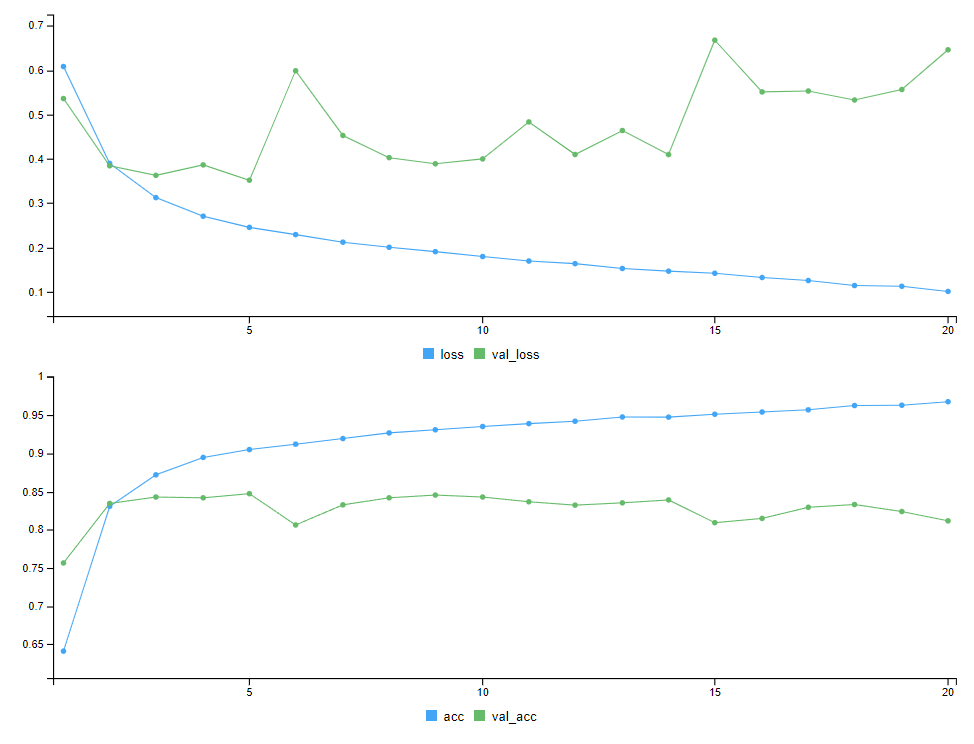
\includegraphics[width=\maxwidth]{lstm_model_2} \caption[Results for second LSTM model]{Results for second LSTM model}\label{fig:lstm_model_2_plot}
\end{figure}

\end{knitrout}
Looking at the results, then we see that the validation accuracy for the last epoch is 0.81, and looking at \ref{fig:lstm_model_2_plot} it can be seen that this is were the accuracy seem to stabilize around already after  a few epochs. 

Now we can try some more minor adjustments to see if we can gain some additional accuracy. we can increase the number of words used to 500. Since this also increases the computational power required, then I will also increase the batch size to 256. Also, we can fine tune the learning rate to decrease after 5 epochs. The reason is that an improper learning rate will result in a model with low effective capacity due to optimization problems. The reason for choosing 5 is since the  previous models seemed to have converged around that point. 

\begin{knitrout}
\definecolor{shadecolor}{rgb}{0.969, 0.969, 0.969}\color{fgcolor}\begin{kframe}
\begin{alltt}
\hlstd{maxlen} \hlkwb{<-} \hlnum{200} \hlcom{#cut off the text after 20 words}
\hlkwd{c}\hlstd{(}\hlkwd{c}\hlstd{(input_train, y_train),} \hlkwd{c}\hlstd{(input_test, y_test))} \hlopt \hlstd{imdb}
\hlstd{input_train} \hlkwb{<-} \hlkwd{pad_sequences}\hlstd{(input_train,} \hlkwc{maxlen} \hlstd{= maxlen)} \hlcom{#load data as list of integers}
\hlstd{input_test} \hlkwb{<-} \hlkwd{pad_sequences}\hlstd{(input_test,} \hlkwc{maxlen} \hlstd{= maxlen)} \hlcom{#turn the list of integers into a 2D integer tensor of shape}

\hlstd{LSTM_model3} \hlkwb{<-} \hlkwd{keras_model_sequential}\hlstd{()} \hlopt
  \hlkwd{layer_embedding}\hlstd{(}\hlkwc{input_dim} \hlstd{=} \hlnum{10000}\hlstd{,} \hlkwc{output_dim} \hlstd{=} \hlnum{16}\hlstd{)} \hlopt
  \hlkwd{layer_lstm}\hlstd{(}\hlkwc{units} \hlstd{=} \hlnum{32}\hlstd{,} \hlkwc{dropout} \hlstd{=} \hlnum{0.2}\hlstd{,} \hlkwc{recurrent_dropout} \hlstd{=} \hlnum{0.2}\hlstd{,} \hlkwc{return_sequences} \hlstd{=} \hlnum{TRUE}\hlstd{)} \hlopt
  \hlkwd{layer_lstm}\hlstd{(}\hlkwc{units} \hlstd{=} \hlnum{32}\hlstd{,} \hlkwc{dropout} \hlstd{=} \hlnum{0.2}\hlstd{,} \hlkwc{recurrent_dropout} \hlstd{=} \hlnum{0.2}\hlstd{)} \hlopt
  \hlkwd{layer_dense}\hlstd{(}\hlkwc{units} \hlstd{=} \hlnum{1}\hlstd{,} \hlkwc{activation} \hlstd{=} \hlstr{"sigmoid"}\hlstd{)}

\hlkwd{summary}\hlstd{(LSTM_model3)}
\end{alltt}
\begin{verbatim}
Model: "sequential_4"
________________________________________________________________________________
 Layer (type)                       Output Shape                    Param #     
================================================================================
 embedding_4 (Embedding)            (None, None, 16)                160000      
 lstm_4 (LSTM)                      (None, None, 32)                6272        
 lstm_3 (LSTM)                      (None, 32)                      8320        
 dense_5 (Dense)                    (None, 1)                       33          
================================================================================
Total params: 174625 (682.13 KB)
Trainable params: 174625 (682.13 KB)
Non-trainable params: 0 (0.00 Byte)
________________________________________________________________________________
\end{verbatim}
\end{kframe}
\end{knitrout}

\begin{knitrout}
\definecolor{shadecolor}{rgb}{0.969, 0.969, 0.969}\color{fgcolor}\begin{kframe}
\begin{alltt}
\hlstd{LSTM_model3} \hlopt \hlkwd{compile}\hlstd{(}
  \hlkwc{optimizer} \hlstd{=} \hlstr{"rmsprop"}\hlstd{,}
  \hlkwc{loss} \hlstd{=} \hlstr{"binary_crossentropy"}\hlstd{,}
  \hlkwc{metrics} \hlstd{=} \hlkwd{c}\hlstd{(}\hlstr{"acc"}\hlstd{)}
\hlstd{)}

\hlstd{Scheduler} \hlkwb{<-} \hlkwa{function}\hlstd{(}\hlkwc{epoch}\hlstd{,} \hlkwc{lr}\hlstd{) \{}
  \hlkwa{if} \hlstd{(epoch} \hlopt{<} \hlnum{5}\hlstd{) \{}
    \hlkwd{return}\hlstd{(lr)}
  \hlstd{\}} \hlkwa{else} \hlstd{\{}
    \hlkwd{return}\hlstd{(lr} \hlopt{*} \hlkwd{exp}\hlstd{(}\hlopt{-}\hlnum{0.1}\hlstd{))}
  \hlstd{\}}
\hlstd{\}}

\hlstd{callback_list} \hlkwb{=} \hlkwd{list}\hlstd{(}\hlkwd{callback_early_stopping}\hlstd{(}\hlkwc{patience} \hlstd{=} \hlnum{5}\hlstd{),}
                     \hlkwd{callback_learning_rate_scheduler}\hlstd{(Scheduler))}

\hlstd{history_LSTM3} \hlkwb{<-} \hlstd{LSTM_model3} \hlopt
  \hlkwd{fit}\hlstd{(}
  \hlstd{input_train, y_train,}
  \hlkwc{epochs} \hlstd{=} \hlnum{20}\hlstd{,}
  \hlkwc{batch_size} \hlstd{=} \hlnum{256}\hlstd{,}
  \hlkwc{validation_split} \hlstd{=} \hlnum{0.2}\hlstd{,}
    \hlkwc{shuffle} \hlstd{=} \hlnum{TRUE}\hlstd{,}
  \hlkwc{callbacks} \hlstd{=callback_list)}
\end{alltt}
\end{kframe}
\end{knitrout}

This ended early due to early stopping. The state with the best results before ending it was:
\begin{knitrout}
\definecolor{shadecolor}{rgb}{0.969, 0.969, 0.969}\color{fgcolor}\begin{kframe}
\begin{alltt}
79/79 [==============================] - 
  51s 648ms/step - loss: 0.1860 - acc: 0.9304 - val_loss: 0.3046 - val_acc: 0.8716 - lr: 7.4082e-04
\end{alltt}
\end{kframe}
\end{knitrout}

Here we see that the validation accuracy has increased to 0.87. The same as before, we can also  plot the entire history. 
\begin{knitrout}
\definecolor{shadecolor}{rgb}{0.969, 0.969, 0.969}\color{fgcolor}\begin{kframe}
\begin{alltt}
\hlstd{knitr}\hlopt{::}\hlkwd{include_graphics}\hlstd{(}\hlstr{"lstm_model_3.png"}\hlstd{)}
\end{alltt}
\end{kframe}
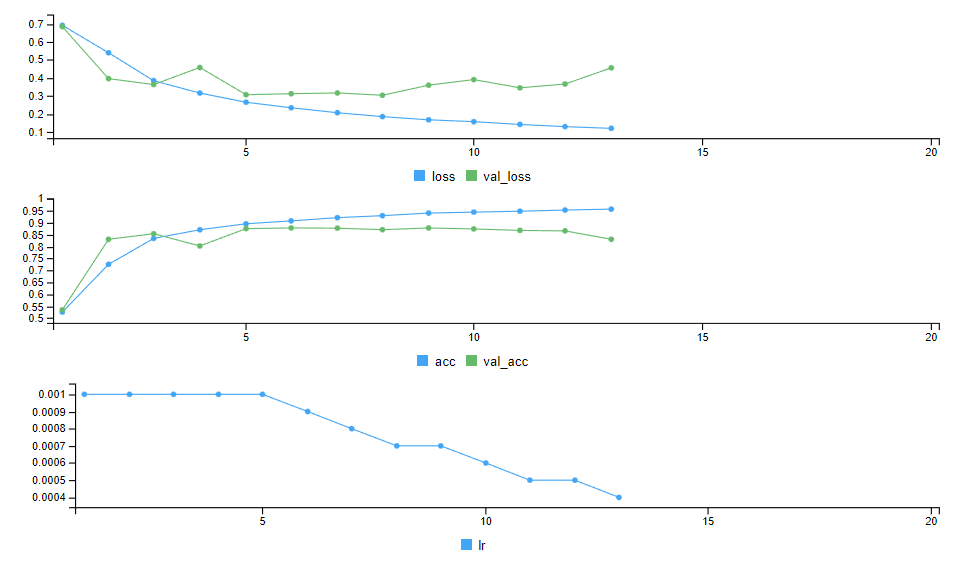
\includegraphics[width=\maxwidth]{lstm_model_3} 
\end{knitrout}

Now lastly, we can run this best-performing model on the test set to make check if we have over fitted on the validation set. 

\begin{knitrout}
\definecolor{shadecolor}{rgb}{0.969, 0.969, 0.969}\color{fgcolor}\begin{kframe}
\begin{alltt}
\hlstd{evaluation} \hlkwb{<-} \hlstd{LSTM_model3} \hlopt \hlkwd{evaluate}\hlstd{(input_test, y_test)}
\end{alltt}
\end{kframe}
\end{knitrout}

\begin{knitrout}
\definecolor{shadecolor}{rgb}{0.969, 0.969, 0.969}\color{fgcolor}\begin{kframe}
\begin{alltt}
782/782 [==============================] - 16s 20ms/step - loss: 0.4716 - acc: 0.8257
\end{alltt}
\end{kframe}
\end{knitrout}
Looking at the results, then the accuracy for the test set was 0.825. Hence this could indicate that the previous model may have overfitted to a certain degree, since this accuracy is lower. 


\end{document}


